\documentclass{beamer}
\usepackage[utf8]{inputenc}

\usetheme{Madrid}
\usecolortheme{default}
\usepackage{extarrows}
\usepackage{amsmath}
\usepackage{extarrows}
\usepackage{amssymb,amsfonts,amsthm}
\usepackage{txfonts}
\usepackage{tkz-euclide}
\usepackage{listings}
\usepackage{adjustbox}
\usepackage{array}
\usepackage{tabularx}
\usepackage{gvv}
\usepackage{lmodern}
\usepackage{circuitikz}
\usepackage{tikz}
\usepackage{graphicx}
\usepackage{amsmath} 

\setbeamertemplate{page number in head/foot}[totalframenumber]

\usepackage{tcolorbox}
\tcbuselibrary{minted,breakable,xparse,skins}

\definecolor{bg}{gray}{0.95}
\DeclareTCBListing{mintedbox}{O{}m!O{}}{%
  breakable=true,
  listing engine=minted,
  listing only,
  minted language=#2,
  minted style=default,
  minted options={%
    linenos,
    gobble=0,
    breaklines=true,
    breakafter=,,
    fontsize=\small,
    numbersep=8pt,
    #1},
  boxsep=0pt,
  left skip=0pt,
  right skip=0pt,
  left=25pt,
  right=0pt,
  top=3pt,
  bottom=3pt,
  arc=5pt,
  leftrule=0pt,
  rightrule=0pt,
  bottomrule=2pt,
  toprule=2pt,
  colback=bg,
  colframe=orange!70,
  enhanced,
  overlay={%
    \begin{tcbclipinterior}
    \fill[orange!20!white] (frame.south west) rectangle ([xshift=20pt]frame.north west);
    \end{tcbclipinterior}},
  #3,
}
\lstset{
    language=C,
    basicstyle=\ttfamily\small,
    keywordstyle=\color{blue},
    stringstyle=\color{orange},
    commentstyle=\color{green!60!black},
    numbers=left,
    numberstyle=\tiny\color{gray},
    breaklines=true,
    showstringspaces=false,
}
\title %optional
{7.4.39}


\author 
{Kartik Lahoti - EE25BTECH11032}



\begin{document}


\frame{\titlepage}
\begin{frame}{Question}
If $\brak{m_i , \frac{1}{m_i}}$ , $m_i > 0 , i = 1, 2,3,4$ are four distinct points on a circle, then show that $m_1m_2m_3m_4 = 1 $
\end{frame}

\begin{frame}{Theoretical Solution}

Let the circle equation be 
\begin{align}
    \norm{\vec{x}}^2 + 2\vec{u}^{\top}\vec{x} + f = 0 
\end{align}

where, $\vec{u} = \myvec{a \\ b}$ with $a$ and $b$ as constants.

Let $\vec{P} = \myvec{m \\ \frac{1}{m}}$ be a arbitrary vector in space.

Putting $\vec{P}$ in the circle , we get 

\begin{align}
    \norm{\vec{P}}^2 + 2\vec{u}^{\top}\vec{P} + f = 0 
\end{align}

\end{frame}

\begin{frame}{Theoretical Solution}
\begin{align}
    m^2 + \frac{1}{m^2} + 2am + \frac{2b}{m} + f = 0
\end{align}
Let,
\begin{align}
  p\brak{m} = m^4 + 2am^3 + fm^2 + 2bm + 1 = 0 \label{eq_1}
\end{align}

\end{frame}

\begin{frame}{Theoretical Solution}
A general polynomial of degree $n$, has companion matrix as

\begin{align}
   \vec{C} = \myvec{0 & 0 & 0 & \cdots & 0 & -c_{0} \\
1 & 0 & 0 & \cdots & 0 & -c_{1} \\
0 & 1 & 0 & \cdots & 0 & -c_{2} \\
0 & 0 & 1 & \cdots & 0 & -c_{3} \\
\vdots & \vdots & \vdots & \ddots & \vdots & \vdots \\
0 & 0 & 0 & \cdots & 1 & -c_{n-1}}
\end{align}

The eigen values of the Companion Matrix $\vec{C}$ are the roots of the polynomial.
\end{frame}
\begin{frame}{Theoretical Solution}
For the question , 
\begin{align}
    \vec{C} = \myvec{0&0&0&-1\\
                     1&0&0&-2b\\
                     0&1&0&-f\\
                     0&0&1&-2a}\\
    \mydet{m\vec{I}-\vec{C}} = p\brak{m}
\end{align}

Here Eigen values of $\vec{C}$ are $m_i$ where $i \in \cbrak{1,2,3,4}$
\end{frame}

\begin{frame}{Theoretical Solution}
Introducing Reversal Matrix 
\begin{align}
    \vec{J} &= \myvec{0&0&0&1\\0&0&1&0\\0&1&0&0\\1&0&0&0} \\ 
    \vec{J}^2 &= \vec{I} \label{eq_2}
\end{align}

The Matrix $\vec{J}$ flips Rows when pre-multiplied and flips column when post-multiplied.
\end{frame}

\begin{frame}{Theoretical Solution}

Then,

\begin{align}
  \mydet{\frac{1}{m}\vec{I}-\vec{J}\vec{C}\vec{J}} = p\brak{\frac{1}{m}}
\end{align}

Since $p\brak{\frac{1}{m}}$ has eigen values $1/m_i$ , we can say 
\begin{align}
    \vec{J}\vec{C}\vec{J} = \vec{C}^{-1} \\
\end{align}
\end{frame}

\begin{frame}{Theoretical Solution}
Taking determinant, using \ref{eq_2}

\begin{align}
    \mydet{\vec{C}} &= \mydet{\vec{C}^{-1}}\\
    \mydet{\vec{C}}^2 &= 1 
\end{align}
\end{frame}
\begin{frame}{Theoretical Solution}
Since $\vec{C}$ is a real companion matrix of a monic quartic whose constant term is $1$ , 

\begin{align}
  \mydet{\vec{C}} &= \brak{-1}^4 1 
\end{align}

Also, 
\begin{align}
  \mydet{\vec{C}} &= m_1m_2m_3m_4
\end{align}
\begin{align}
    \therefore m_1m_2m_3m_4 &= 1 
\end{align}

Hence Proved
\end{frame}


\begin{frame}[fragile]
    \frametitle{C Code - To find Solution of Circle and Hyperbola }
    \begin{lstlisting}
#include <math.h>
double calc(double *X , double *Y , double c, double r)
{
    double temp1 , temp2 ,prod; 
    temp1 = (r*r + sqrt(pow(r,4) - 4 *  pow(c,4)))/2;
    temp2 = (r*r - sqrt(pow(r,4) - 4 *  pow(c,4)))/2; 
    X[0] = sqrt(temp1);
    X[1] = -sqrt(temp1);
    X[2] = sqrt(temp2);
    X[3] = -sqrt(temp2);
    prod = pow(sqrt(temp1),2) * pow(sqrt(temp2),2);
    for(int i = 0 ; i< 4 ; i++)
        Y[i] = c*c/X[i] ;
    return prod;
}


    \end{lstlisting}
\end{frame}

\begin{frame}[fragile]
    \frametitle{C Code - Generate Circle }
    \begin{lstlisting}
void circle_gen(double *X , double *Y , double *P, int n , double r)
{
 
    for (int i  = 0 ; i < n ; i++ )
    {
        double theta = 2.0 * M_PI * i / n ; 
        X[i] = P[0] + r * cos(theta);
        Y[i] = P[1] + r * sin (theta); 
    }   
}

\end{lstlisting}
\end{frame}
\begin{frame}[fragile]
    \frametitle{C Code - To generate Hyperbola }
    \begin{lstlisting}
	
void points_gen (double *X , double a , double b , int n )
{
    double temp = (b - a )/(double)n ; 
    for (int i = 0 ; i <= n ; i++ )
    {
        X[i] = a + temp * i ; 
    }
}

void hyper_gen (double *X , double *Y , double c , int n )
{
    for(int i = 0; i < n ;i++)
    {
        Y[i] = c*c/X[i];
    }
}


\end{lstlisting}
\end{frame}


\begin{frame}[fragile]
    \frametitle{Python Code - 1}
    \begin{lstlisting}
import ctypes as ct
import numpy as np
import matplotlib.pyplot as plt

handc1 = ct.CDLL("./generator.so")

handc1.circle_gen.argtypes = [
    ct.POINTER(ct.c_double),
    ct.POINTER(ct.c_double),
    ct.POINTER(ct.c_double),
    ct.c_int,
    ct.c_double
]

handc1.circle_gen.restype = None

\end{lstlisting}
\end{frame}

\begin{frame}[fragile]
    \frametitle{Python Code - 1}
    \begin{lstlisting}
O = np.zeros(2 , dtype = np.float64).reshape(-1,1)
X_cic = np.zeros(200, dtype = np.float64).reshape(-1,1)
Y_cic = np.zeros(200, dtype = np.float64).reshape(-1,1)

handc1.circle_gen(
    X_cic.ctypes.data_as(ct.POINTER(ct.c_double)),
    Y_cic.ctypes.data_as(ct.POINTER(ct.c_double)),
    O.ctypes.data_as(ct.POINTER(ct.c_double)),
    200 , 3 )
handc1.points_gen.argtypes = [
    ct.POINTER(ct.c_double),
    ct.c_double,
    ct.c_double,
    ct.c_int]
\end{lstlisting}
\end{frame}


\begin{frame}[fragile]
    \frametitle{Python Code - 1}
    \begin{lstlisting}
handc1.points_gen.restype = None


pt = 400
X_hyper_p = np.zeros(pt,dtype=np.float64).reshape(-1,1)
Y_hyper_p = np.zeros(pt,dtype=np.float64).reshape(-1,1)

handc1.points_gen(
    X_hyper_p.ctypes.data_as(ct.POINTER(ct.c_double)),
    0.1,
    30,
    pt 
)

\end{lstlisting}
\end{frame}

\begin{frame}[fragile]
    \frametitle{Python Code - 1}
    \begin{lstlisting}
X_hyper_n = np.zeros(pt,dtype=np.float64).reshape(-1,1)
Y_hyper_n = np.zeros(pt,dtype=np.float64).reshape(-1,1)

handc1.points_gen(
    X_hyper_n.ctypes.data_as(ct.POINTER(ct.c_double)),
    -30,-0.1,pt
)
handc1.hyper_gen.argtypes = [
    ct.POINTER(ct.c_double),
    ct.POINTER(ct.c_double),
    ct.c_double,
    ct.c_int 
]
\end{lstlisting}
\end{frame}


\begin{frame}[fragile]
    \frametitle{Python Code - 1}
    \begin{lstlisting}
handc1.hyper_gen.restype = None

handc1.hyper_gen(
    X_hyper_p.ctypes.data_as(ct.POINTER(ct.c_double)),
    Y_hyper_p.ctypes.data_as(ct.POINTER(ct.c_double)),
    1,pt
)

handc1.hyper_gen(
    X_hyper_n.ctypes.data_as(ct.POINTER(ct.c_double)),
    Y_hyper_n.ctypes.data_as(ct.POINTER(ct.c_double)),
    1,pt
)

\end{lstlisting}
\end{frame}

\begin{frame}[fragile]
    \frametitle{Python Code - 1}
    \begin{lstlisting}
plt.figure()
plt.plot(X_cic,Y_cic,"blue",label= "Circle")
plt.plot(X_hyper_p,Y_hyper_p,"red",label="Rectangular Hyperbola")
plt.plot(X_hyper_n,Y_hyper_n,"red")

handc2 = ct.CDLL("./func.so")

handc2.calc.argtypes = [
    ct.POINTER(ct.c_double),
    ct.POINTER(ct.c_double),
    ct.c_double,
    ct.c_double
]
\end{lstlisting}
\end{frame}


\begin{frame}[fragile]
    \frametitle{Python Code - 1}
    \begin{lstlisting}
handc2.calc.restype = ct.c_double

x = np.zeros(4,dtype=np.float64)
y = np.zeros(4,dtype=np.float64)

prod = handc2.calc(
    x.ctypes.data_as(ct.POINTER(ct.c_double)),
    y.ctypes.data_as(ct.POINTER(ct.c_double)),
    1 , 3
)
print("m_1m_2m_3m_4 = ",prod)
plt.scatter(x,y)
vert_labels = [r'$m_1$',r'$m_2$',r'$m_3$',r'$m_4$']

\end{lstlisting}
\end{frame}

\begin{frame}[fragile]
    \frametitle{Python Code - 1}
    \begin{lstlisting}
for i, txt in enumerate(vert_labels):
    plt.annotate(f'({txt},1/{txt})',
                 (x[i], y[i]),
                 textcoords="offset points",
                 xytext=(10,-15),
                 ha='center')

plt.xlabel('$x$')
plt.ylabel('$y$')
\end{lstlisting}
\end{frame}


\begin{frame}[fragile]
    \frametitle{Python Code - 1}
    \begin{lstlisting}
plt.legend(loc='best')
plt.grid() 
plt.axis('equal')
plt.xlim([-10/2,10/2])
plt.ylim([-10/2,10/2])
plt.title("7.4.39")
plt.axhline(0, color='black', linewidth=0.7)
plt.axvline(0, color='black', linewidth=0.7)
plt.savefig("../figs/graph1.png")
plt.show()


\end{lstlisting}
\end{frame}

\begin{frame}[fragile]
    \frametitle{Python Code - 2}
    \begin{lstlisting}
import math
import sys
sys.path.insert(0, '/home/kartik-lahoti/matgeo/codes/CoordGeo')
import numpy as np
import numpy.linalg as LA
import matplotlib.pyplot as plt
import matplotlib.image as mpimg

from conics.funcs import *
\end{lstlisting}
\end{frame}

\begin{frame}[fragile]
    \frametitle{Python Code - 2}
    \begin{lstlisting}
def intersect_hyperbola_circle(c, r):
    #Find intersection points of xy = c^2 and x^2 + y^2 = r^2
    # Coefficients for quadratic in X = x^2
    # X^2 - r^2*X + c^4 = 0
    coeffs = [1, -r**2, c**4]
    roots = np.roots(coeffs)

    points = []
    for X in roots:
        if np.isreal(X) and X >= 0:   # valid x^2
            x_vals = [np.sqrt(X).real, -np.sqrt(X).real]
            for x in x_vals:
                if x != 0:  # avoid division by zero
                    y = c**2 / x
                    points.append((x, y))
    return points

\end{lstlisting}
\end{frame}

\begin{frame}[fragile]
    \frametitle{Python Code - 2}
    \begin{lstlisting}
lt = intersect_hyperbola_circle(1,3)
inter1 = np.array([lt[0][0] , lt[0][1]]).reshape(-1,1)
inter2 = np.array([lt[1][0] , lt[1][1]]).reshape(-1,1)
inter3 = np.array([lt[2][0] , lt[2][1]]).reshape(-1,1)
inter4 = np.array([lt[3][0] , lt[3][1]]).reshape(-1,1)
prod = lt[0][0] * lt[1][0] * lt[2][0] * lt[3][0] 
print('m_1m_2m_3m_4 = ',prod)
# xy = c^2 
y_n = np.linspace(-30, -0.1 , 400)
y_n = y_n[y_n!=0]
x_n = 1**2/y_n 
 
y_p = np.linspace(0.1, 30 , 400)
y_p = y_p[y_p!=0]
x_p = 1**2/y_p
\end{lstlisting}
\end{frame}
\begin{frame}[fragile]
    \frametitle{Python Code - 2}
    \begin{lstlisting}
plt.figure()
plt.plot(x_p,y_p,"r-",label="Rectangular Hyperbola")
plt.plot(x_n,y_n,"r-")
O = np.zeros(2,dtype=np.float64).reshape(-1,1)
x_circ = circ_gen(O,3)
plt.plot(x_circ[0,:],x_circ[1,:],"blue",label="Circle")

coords = np.block([[inter1,inter2,inter3,inter4]])
plt.scatter(coords[0,:],coords[1,:])
vert_labels = [r'$m_1$',r'$m_2$',r'$m_3$',r'$m_4$']
\end{lstlisting}
\end{frame}
\begin{frame}[fragile]
    \frametitle{Python Code - 2}
    \begin{lstlisting}
for i, txt in enumerate(vert_labels):
    plt.annotate(f'({txt},1/{txt})',(coords[0,i], coords[1,i]),            textcoords="offset points",xytext=(10,-15),ha='center')

plt.xlabel('$x$')
plt.ylabel('$y$')
plt.legend(loc='best')
plt.grid() 
plt.axis('equal')
plt.xlim([-10/2,10/2])
plt.ylim([-10/2,10/2])
plt.title("7.4.39")
plt.axhline(0, color='black', linewidth=0.7)
plt.axvline(0, color='black', linewidth=0.7)
plt.savefig("../figs/graph2.png")
plt.show()
\end{lstlisting}
\end{frame}

 \begin{frame}{Plot}
    \centering
    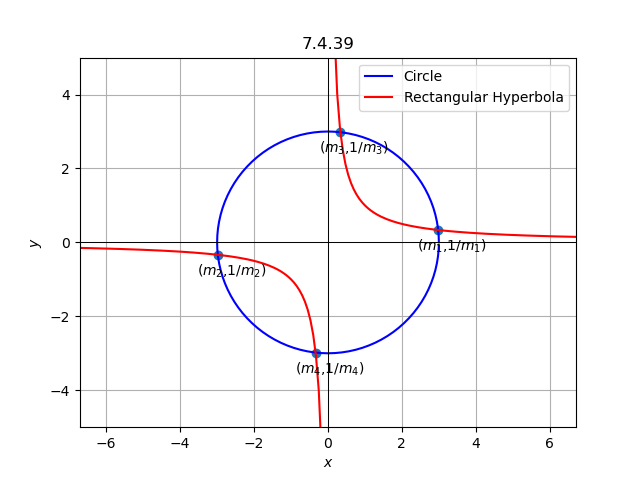
\includegraphics[width=\columnwidth, height=0.8\textheight, keepaspectratio]{../figs/graph1.png}   
\end{frame}

\end{document}
